% Name: Indifference curves and a budget line
% Description: Three indifference curves for two goods and the budget line that touches the highest one it can reach, at the consumer's best choice.
% Tags: indifference curves, budget constraint, utility, consumer choice

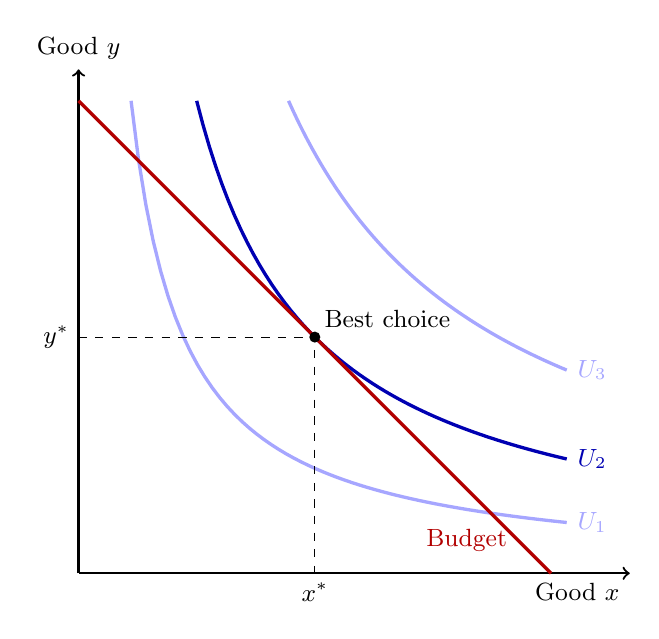
\begin{tikzpicture}[every node/.style={font=\small}]
  \draw[->, thick] (0,0) -- (7,0) node[below left] {Good $x$};
  \draw[->, thick] (0,0) -- (0,6.4) node[above] {Good $y$};
  % The curves xy = 4, 9, and 16; the budget line x + y = 6 touches the middle one at (3,3).
  \foreach \u/\c/\name in {4/blue!35/U_1, 9/blue!70!black/U_2, 16/blue!35/U_3}
    \draw[very thick, \c, domain={\u/6}:6.2, samples=60] plot (\x, {\u/\x}) node[right] {$\name$};
  \draw[very thick, red!70!black] (0,6) -- (6,0) node[pos=0.93, left] {Budget};
  \draw[dashed] (0,3) node[left] {$y^*$} -| (3,0) node[below] {$x^*$};
  \fill (3,3) circle (2pt) node[above right] {Best choice};
\end{tikzpicture}
